%%%%%%%%%%%%%%%%%%%%%%%%%%%%%%%%%%%%%%%%%
% University Assignment Title Page 
% LaTeX Template
% Version 1.0 (27/12/12)
%
% This template has been downloaded from:
% http://www.LaTeXTemplates.com
%
% Original author:
% WikiBooks (http://en.wikibooks.org/wiki/LaTeX/Title_Creation)
%
% License:
% CC BY-NC-SA 3.0 (http://creativecommons.org/licenses/by-nc-sa/3.0/)
% 
% Instructions for using this template:
% This title page is capable of being compiled as is. This is not useful for 
% including it in another document. To do this, you have two options: 
%
% 1) Copy/paste everything between \begin{document} and \end{document} 
% starting at \begin{titlepage} and paste this into another LaTeX file where you 
% want your title page.
% OR
% 2) Remove everything outside the \begin{titlepage} and \end{titlepage} and 
% move this file to the same directory as the LaTeX file you wish to add it to. 
% Then add \input{./title_page_1.tex} to your LaTeX file where you want your
% title page.
%
%%%%%%%%%%%%%%%%%%%%%%%%%%%%%%%%%%%%%%%%%
%\title{Title page with logo}
%----------------------------------------------------------------------------------------
%	PACKAGES AND OTHER DOCUMENT CONFIGURATIONS
%----------------------------------------------------------------------------------------
\documentclass[12pt]{article}
\usepackage[spanish]{babel}
\usepackage[utf8x]{inputenc}
\usepackage{amsmath}
\usepackage{graphicx}
\usepackage[colorinlistoftodos]{todonotes}
\usepackage{makeidx}
\usepackage[colorlinks=true,linkcolor=black,anchorcolor=black,citecolor=black,filecolor=black,menucolor=black,runcolor=black,urlcolor=blue]{hyperref}
\usepackage{color}
\usepackage{caption}
\usepackage{etoolbox}
\usepackage{fancybox}
\usepackage{enumitem}
\usepackage{listings}
\lstset{
	language=sh,
	breaklines=true,
	breakatwhitespace=true,
	basicstyle=\ttfamily,
	showstringspaces=false,
	columns=fullflexible-
}    	

\newcommand{\icon}[1]{\includegraphics[height=18pt]{#1}}
\robustify{\icon}
\makeindex
\graphicspath{{./img/}}

\begin{document}

\renewcommand\indexname{Índice}
\begin{titlepage}

\newcommand{\HRule}{\rule{\linewidth}{0.5mm}} % Defines a new command for the horizontal lines, change thickness here

\center % Center everything on the page
 
%----------------------------------------------------------------------------------------
%	HEADING SECTIONS
%----------------------------------------------------------------------------------------

\textsc{\LARGE Facultad de Informática}\\[1.5cm] % Name of your university/college
\textsc{\large Adrián García García}\\[0.5cm] % Minor heading such as course title

%----------------------------------------------------------------------------------------
%	TITLE SECTION
%----------------------------------------------------------------------------------------

\HRule \\[0.4cm]
{ \huge \bfseries Arquitecturas Cloud y microservicios}\\[0.4cm] % Title of your document
\HRule \\[1.5cm]
 
%----------------------------------------------------------------------------------------
%	AUTHOR SECTION
%----------------------------------------------------------------------------------------


% If you don't want a supervisor, uncomment the two lines below and remove the section above
%\Large \emph{Author:}\\
%John \textsc{Smith}\\[3cm] % Your name

%----------------------------------------------------------------------------------------
%	DATE SECTION
%----------------------------------------------------------------------------------------

{\large \today}\\[2cm] % Date, change the \today to a set date if you want to be precise

%----------------------------------------------------------------------------------------
%	LOGO SECTION
%----------------------------------------------------------------------------------------


\includegraphics[width=4cm,keepaspectratio]{logo.png}
 
%----------------------------------------------------------------------------------------

\vfill % Fill the rest of the page with whitespace



\captionsetup[figure]{labelformat=empty,justification=raggedright,singlelinecheck=false}
% Include image from images directory
\begin{figure}[h]

        
\includegraphics[width=2cm,keepaspectratio]{cc-by-sa.png}
        \label{fig:by-sa}
        \caption{ This work is licensed under a \href{https://creativecommons.org/licenses/by/4.0/legalcode}{CC-BY-SA 4.0 License}.}

\end{figure}

\end{titlepage}

\tableofcontents
\clearpage

\begin{abstract}
Este trabajo tiene como objetivo exponer y profundizar en los conceptos expuestos en una conferencia optativa que tuvo lugar durante la semana de la informática de 2017. Los ponentes fueron dos ingenieros de la empresa GMV (Ricardo de Castro y Roberto Galán). En concreto, el nombre de la conferencia era el siguiente: Despliegue automático de arquitecturas escalables basadas en microservicios sobre el Cloud de Google (23 de Febrero, 11-14 horas). Conviene puntualizar que al final no usaron la plataforma de Google, sino que se basaron en Amazon Web Services y Docker Swarm para desplegar una aplicación web que se basaba en el uso de microservicios para su funcionamiento. Al mismo tiempo, hablaron de un concepto que está muy de moda últimamente como es el enfoque \emph{DevOps}, también está relacionado con el despliegue rápido y eficiente de código en la nube, la automatización de procesos de desarrollo (\emph{testing}, recogida de métricas, despliegue, etc.) y las metodologías ágiles.
\end{abstract}

\section{Introducción}\label{sec:intro}

Durante la conferencia, se hizo especial hincapié en las necesidades de los clientes y las características que estos exigen en una aplicación de carácter empresarial que se ejecuta en la nube. Los requisitos más destacados son los siguientes:

\begin{itemize}
\item \textbf{Fiabilidad}. El funcionamiento de las aplicaciones web está íntimamente relacionado con la imagen que las grandes empresas tienen en la sociedad, si una tienda de comercio electrónico se cae durante una hora puede suponer pérdidas millonarias para la empresa y acarrea el riesgo de que sus clientes dejen de confiar en ella y se pasen a la competencia. Debido a esto, los clientes esperan que su aplicación tenga el mínimo número de errores posibles. Uno de los aspectos más importantes en este sentido es que se haga un proceso meticuloso de \emph{testing} y validación antes de publicar una aplicación, priorizando las partes más críticas del sistema y que pueden suponer un cuello de botella para la misma.
\item \textbf{Recuperación instantánea ante fallos} (\emph{Zero Down Time}\cite{zdwt}). En caso de que la aplicación llegue a fallar, lo que es imposible de evitar al completo, es necesario minimizar el tiempo en el que no se provee un servicio. Asegurar un tiempo mínimo de recuperación supone un desafío importante cuando una máquina física actúa como el punto de fallo único de la aplicación. Sin embargo, el hecho de tener una aplicación desplegada en contenedores virtuales, nos facilita en gran medida asegurar un sistema tolerante a fallos. Este sistema debe constar de ciertas características, entre las que se destacan:
\begin{itemize}
\item Disponer de un \textbf{cluster de máquinas} configurado.
\item Aplicar técnicas de \textbf{replicación y balanceo de carga}.
\item Tener montado un \textbf{volumen compartido de datos} que permita a diferentes máquinas acceder a las imágenes que utilizan las máquinas virtuales. Por ejemplo, \emph{Network File System} (\textbf{NFS}).
\end{itemize}
\begin{figure}
\centering
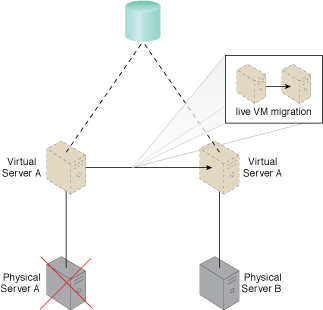
\includegraphics[width=0.5\textwidth]{spof.png}
\caption{\label{fig:zerodt}Esquema de recuperación ante fallos.}
\end{figure}
Cómo se puede observar en la Figura~\ref{fig:zerodt}, cuando el servidor físico A falla, se desencadena una migración del contenedor virtual al servidor B. Lo que debería ocurrir sin complicaciones en caso de que el volumen de datos compartido por red siga disponible y solo haya ocurrido un problema aislado en la máquina A. En general, el demonio encargado de vigilar el correcto funcionamiento de los nodos se denomina \textit{watchdog} y su funcionamiento se basa en el intercambio periódico de mensajes con los nodos del cluster para intercambiar información del estado del servicio (\textit{keepalive o hearbeat}).
\item \textbf{Tiempo rápido de despliegue}. Uno de los problemas más extendidos en el ámbito de las aplicaciones empresariales de elevada complejidad es que la aplicación puede tener muchas dependencias entre diferentes componentes, lo que hace difícil realizar un despliegue limpio y sin errores. Se ponía como ejemplo el clásico problema de que en el entorno de desarrollo funciona todo perfectamente, pero cuando se traslada a producción deja de hacerlo y cada equipo le echa la culpa a otro.
\item \textbf{Escalabilidad}. Los servicios pueden recibir grandes picos de tráfico y deben ser capaces de responder ante los mismos sin errores. Es evidente que la optimización de cada componente de la aplicación es un aspecto importante, pero además se debe diseñar un sistema capaz de balancear la carga y aumentar la dedicación de recursos replicando sus unidades de cómputo para responder ante los incrementos en demanda. Esto es relativamente fácil de hacer en entornos cloud o con soluciones de virtualización como Docker.
\end{itemize}

Este trabajo está estructurado de la siguiente forma, en la Sección~\ref{sec:cloud} se realizará una exposición de diferentes conceptos que se utilizan en \emph{Cloud Computing}. A continuación se introducirá el paradigma de las arquitecturas orientadas a servicios (SOA) en la Sección~\ref{sec:soa}. Más adelante se introducirá la herramienta de contenedores Docker (Sección~\ref{sec:docker}), con la que se pueden construir de forma sencilla diferentes tipos de aplicaciones basadas en microservicios. Para finalizar, en la Sección~\ref{sec:conclu} presentaré una serie de opiniones personales que se han originado a partir de la conferencia y de la investigación posterior realizada.

\section{Cloud Computing}\label{sec:soa}
A continuación se presentarán diferentes conceptos utilizados en el diseño y construcción de aplicaciones que se ejecutan en la nube, comúnmente conocido como \emph{Cloud Computing}.

\section{Arquitectura orientada a servicios}\label{sec:soa}
El paradigma de creación de arquitecturas orientadas a servicios, comúnmente conocido como SOA (\textbf{Service Oriented Architecture}), trata de definir aplicaciones basadas en el uso de una \textbf{colección servicios que pueden trabajar de forma autónoma}, pero que también intercambian mensajes y se coordinan para cumplir una funcionalidad más compleja. Se parte del concepto de servicio, que es una funcionalidad bien definida, autocontenida y que no depende del contexto o estado de otros servicios. Por ejemplo, validar un cliente en la aplicación o proveer datos sobre el funcionamiento de la misma. La división en servicios tiene las ventajas de que la realización de \textit{tests} y la corrección de errores se puede realizar de una forma mucho más precisa, y no es necesario cambiar la aplicación completa para corregir fallos o introducir nuevas funcionalidades.

Para implementar una arquitectura orientada a servicios de forma eficiente, es necesario tener en cuenta una serie de conceptos y estrategias de diseño:
\begin{itemize}
\item Tener claro un \textbf{conjunto de servicios} que se quieran proveer a nuestros clientes o incluso de forma interna en la organización.
\item Añadir una serie de procesos de \textbf{orquestación}, \textbf{balanceo de cargas} y de \textbf{recolección de métricas} para asegurar el buen funcionamiento de los mismos.
\item Aplicar un conjunto de patrones de diseño que permita realizar un \textbf{diseño modular}, que tenga una buena \textbf{encapsulación} de los componentes, que asegure el \textbf{aislamiento}, la \textbf{reusabilidad} y la \textbf{escalabilidad}.
\item Utilizar un modelo de programación compatibles con diferentes estándares de comunicación y que sea soportado por múltiples tecnologías, por ejemplo, los \textbf{servicios REST}.
\end{itemize}

\begin{figure}
\centering
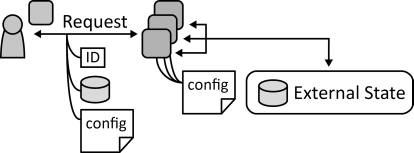
\includegraphics[width=0.5\textwidth]{stateless.png}
\caption{\label{fig:scomm}Peticiones del cliente con estado almacenado fuera de los componentes\cite{sless}.}
\end{figure}

\subsection{Comunicación}\label{sec:intro}
En una arquitectura orientada a servicios uno de los aspectos más importantes es la comunicación, ya sea entre los propios componentes de nuestra aplicación o los métodos de nuestra API que exponemos al público. Los servicios de una aplicación distribuída pueden estar alojados en diferentes máquinas, lo que hace necesario que el estado de nuestra aplicación sea almacenado de forma externa a los componentes, estos se conocen como \textbf{Stateless Components}  (puede verse un esquema en la Figura~\ref{fig:scomm}). Una de las técnicas más habituales para implementarlos es \textbf{incluir la información de estado en las peticiones} que recibe cada componente, otra forma de hacerlo sería transmitirla en los mensajes \emph{keepalive} enviados por los procesos de orquestación.

En este contexto que requiere una comunicación entre múltiples componentes sin ninguna comunicación previa de esquemas de datos, como sí era necesario con protocolos SOAP o XML, podemos destacar la utilidad de las APIs REST por las siguientes características:

\begin{itemize}
\item Representan un \textbf{protocolo cliente/servidor sin estado}.
\item \textbf{ Facilitan la portabilidad} y la comunicación entre diferentes plataformas y lenguajes, ya que se basan en el \textbf{protocolo HTTP} y el uso de sus verbos: POST, GET, PUT y DELETE.
\item Permiten \textbf{exponer recursos de forma sencilla} diferentes  mediante las URI (Unique Resource Identifier).
\item Ofrecen una gran \textbf{flexibilidad para transmitir diferentes tipos de datos}: html, json, text, xml, jpeg, etc.
\end{itemize}

\subsection{Microservicios}\label{sec:micro}
%\subsection{Subsections}\index{Section}
\begin{figure}
\centering
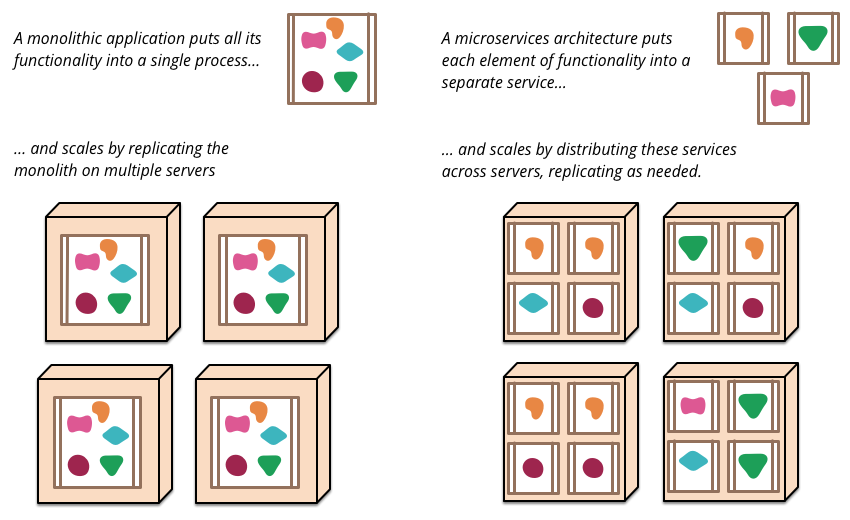
\includegraphics[width=0.9\textwidth]{sketch.png}
\caption{\label{fig:msv}Aplicación monolítica VS microservicios.}
\end{figure}

Las aplicaciones monolíticas se despliegan como un solo bloque de frontend, lógica de negocio y acceso a datos. Si existe un cuello de botella en sólo un elemento del sistema necesitaríamos desplegar varias instancias de la aplicación completa y aplicar algún tipo de balanceo de carga para poder mejorar la latencia de respuesta. Esta es una solución pésima, ya que desperdicia recursos y no resulta eficiente para incrementar el rendimiento.

Como se puede apreciar en la Figura~\ref{fig:msv}, las aplicaciones diseñadas usando microservicios permiten escalar aquellas partes de la aplicación que representen un cuello de botella. Se basa en el concepto de arquitecturas SOA pero dividida aún más en cada dominio (Productos, Empleados, Ventas…). Los componentes pueden ser atómicos o compuestos, que agrupan varios dominios.

Las principales ventajas que aportan el uso de microservicios son las siguientes:
\begin{itemize}
\item La división de las aplicaciones en microservicios nos permite hacer una mayor \textbf{reutilización de componentes} en otras aplicaciones. Varios proyectos suelen compartir una lógica de negocio o de acceso a datos similar, y el diseño modular de los microservicios nos aporta una gran flexibilidad para adaparlos a otros problemas.
\item Como ya mencionamos anteriormente, aporta una gran \textbf{mejora en la escalabilidad del sistema} en función de nuestras necesidades.
\item El proceso de \textbf{mantenimiento se simplifica} enormemente, ya que los componentes sin estado interno permiten reducir el acomplamiento y es más sencillo detectar y resolver los problemas en un único componente sin detener al completo el servicio.
\item El sistema es \textbf{resistente a fallos} ya que, a diferencia de las aplicaciones monolíticas, el fallo de un componente no supone necesariamente el fallo de la aplicación.
\end{itemize}

Desplegar suele resultar el paso más complicado en este tipo de aplicaciones que en las arquitecturas monolíticas convencionales, es necesario levantar múltiples servicios que suelen presentar interdependencias y , por lo tanto, requieren que se realice un orden de arranque concreto. Existe una serie de servicios de código abierto que permiten gestionar los diferentes microservicios y las interacciones que presentan. Algunos de los más usados pertenecen al framework Spring Cloud de Netflix:
\begin{itemize}
\item Eureka: Service Discovery.
\item Zuul: Proxy.
\item Ribbon: Load Balancer.
\end{itemize}



\vspace{1cm}
\section{Docker \icon{docker.png}}\label{sec:docker}
Es una tecnología de virtualización que permite definir aplicaciones autocontenidas. Se basa en el concepto de contenedores, se tratan de entornos de ejecución portables y aislados de la máquina anfitriona. Estos contenedores incluyen todas las librerías y binarios necesarios para el despliegue de una aplicación. Esto permite definir contenedores ligeros de forma eficiente, que tienen todo lo necesario para que una aplicación se ejecute y que tras su despliegue no se oiga la típica excusa de: 'En mi máquina funcionaba'.

\begin{figure}
\centering
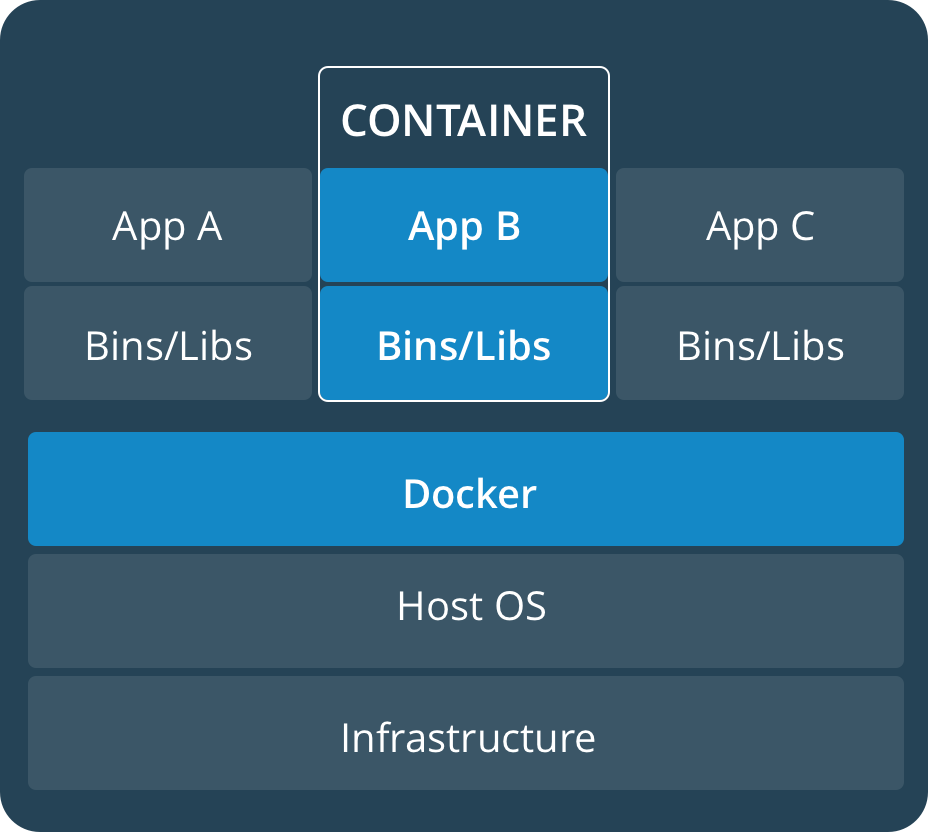
\includegraphics[width=0.4\textwidth]{container.png}
\caption{\label{fig:cont}Infraestructura de un contenedor.}
\end{figure}

A diferencia de las máquinas virtuales convencionales, las tecnologías de contenedores como Docker no incluyen un sistema operativo completo en su imágen, tan solo las librerías y configuraciones necesarias para su funcionamiento (se puede observar un esquema en la Figura~\ref{fig:cont}). Esto permite mejorar la eficiencia al no existir la sobrecarga que supone la interacción de las máquinsa virtuales con el sistema operativo huésped(guest), ya que Docker es capaz de realizar una interacción directa con el Kernel Linux de la máquina anfitrión(host).

Algunas características destacadas sobre Docker en la conferencia son las siguientes: es portable, ligero, automatizable, autocontenido, aislado(ofrece entorno de desarrollo que se comporta a modo de \textit{sandbox}), agiliza el despliegue y el mantenimiento.

Con muchos contenedores pueden aparecer problemas de coordinación, para solucionarlos se utilizan balanceadores de carga o administradores (también conocidos como orquestadores). Algunos de los más conocidos son:
\begin{itemize}
\item Kubernetes (Google)
\item Amazon Web Services ECS
\item Docker Swarm
\end{itemize}

\begin{itemize}[label=\textdollar]
\item \begin{lstlisting}
docker node inspect worker1 | grep IDdocker node update --label-add type=master 18yrb7m650umx738rtevojpqy
\end{lstlisting}
\end{itemize}



\section{DevOps}
%\todo[inline, color=green!40]{This is an inline comment.}

Otro de los conceptos introducidos en la conferencia es el de DevOps (el término proviene del acrónimo inglés formado por \textit{Development y Operations}), es un concepto que ha atraído un interés creciente en el ámbito de la gestión de proyectos y la ingeniería del Software durante la última década. Recibe una gran influencia de las metodologías ágiles de desarrollo y propone una mejora de la comunicación entre los equipos de desarrollo y operaciones. A lo largo de la historia, se ha producido un conflicto entre ambos equipos que surge de forma natural de sus roles, en el área de desarrollo se intenta introducir nueva funcionalidad mientras que el equipo de operaciones crea estabilidad y se ocupa de resolver errores. 

Las técnicas de DevOps se basan en la creación de una cultura común entre ambos equipos, que se aproveche al máximo de la automatización de procesos, la obtención de métricas que permita guiar la toma de decisiones y la integración de ambos equipos de forma que participen en todo el ciclo de vida del proyecto(diseño, desarrollo, mantenimiento…).

Una de las herramientas más utilizadas para automatizar las actividades del ciclo de vida del Software es Jenkins. Esta herramienta permite definir tareas para automatizar el proceso de compilación, \textit{testing}, despliegue y recopilación de métricas. Otras herramientas que pueden de resultar de utilidad son SonarQube(Testing de calidad de código) y NexusOSS(Gestor de dependencias y artefactos).

% -- TABLE --
%\begin{table}
%\centering
%\begin{tabular}{l|r}
%Item & Quantity \\\hline
%Widgets & 42 \\
%Gadgets & 13
%\end{tabular}
%\caption{\label{tab:widgets}An example table.}
%\end{table}

\section{Conclusiones}\label{sec:conclu}


\begin{thebibliography}{1}
%\bibitem{key} description. \href{https://...}{Enlace}
\bibitem{cloudpatts}\textbf{Cloud Computing Patterns, Springer (2014)}. \textit{Fundamentals to Design, Build, and Manage Cloud Applications}. Authors: Christoph Fehling, Frank Leymann, Ralph Retter, Walter Schupeck and Peter Arbitter.
\bibitem{reliab}\href{https://blogs.microsoft.com/microsoftsecure/2012/09/12/fundamentals-of-cloud-service-reliability/}{Fundaments of Cloud Service Reliability}, Microsoft Secure Blog.
\bibitem{zdwt}\href{http://cloudpatterns.org/design_patterns/zero_downtime}{Zero Downtime}, cloudpatterns.org.
\bibitem{wscom}\href{http://www.service-architecture.com/articles/web-services/web_services_explained.html}{Web Services Explained} (Communication). service-architecture.com.
\bibitem{ibmsoa}\href{https://www-01.ibm.com/software/solutions/soa/}{Service Oriented Architecture}: simply good design. ibm.com.
\bibitem{sless}\href{http://www.cloudcomputingpatterns.org/stateless_component/}{Stateless Component, cloudcomputingpatterns.org}
\bibitem{restapi}\href{https://bbvaopen4u.com/es/actualidad/api-rest-que-es-y-cuales-son-sus-ventajas-en-el-desarrollo-de-proyectos}{API REST: ventajas.}  bbvaopen4u.com.
\end{thebibliography}

\end{document}